\newpage
\genHeader
\hypertarget{codeGen common}{} 
\section{Code generation}

Now that you've worked through the specifics of your syntax, lets have a brief discussion on code generation.

The Ecore model is used to drive a code generator that maps the model to Java interfaces and classes. The generated Java code that represents the model is often
referred to as a repository. This is the reason why we refer to such projects as repository projects. A repository can be viewed as an adapter that enables
building and manipulating concrete instances of a specific model via a programming language such as Java. This is why we indicate repository projects using a
cute adapter/plug symbol on the project folder.

If you take a careful look at the code structure in \texttt{gen} (Fig.~\ref{eclipse:structureGen}), you'll find a \texttt{FooImpl.java} for every
\texttt{Foo.java}. Indeed, the subpackage \texttt{.impl} contains Java classes that implement the interfaces in the parent package. Although this might strike
you as unnecessary (why not merge interface and implementation for simple classes?), this consequent separation in interfaces and implementation allows for a
clean and relatively simple mapping of Ecore to Java, even in tricky cases such as multiple inheritance (allowed and very common in Ecore models). A further
package \texttt{.util} contains some auxiliary classes such as a factory for creating instances of the model.

 \begin{figure}[htbp]
  \centering
  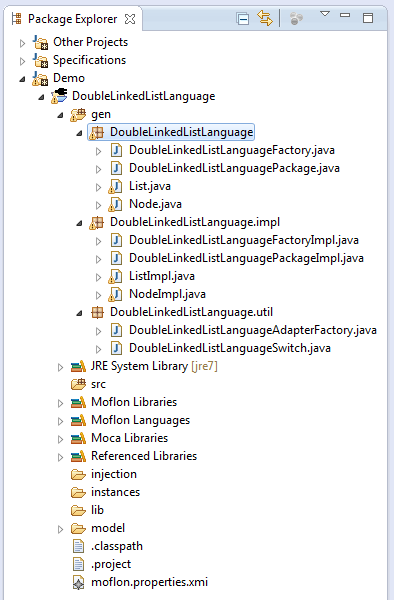
\includegraphics[width=0.45\textwidth]{eclipse_structureGen}
  \caption{\texttt{Gen} package structure}
  \label{eclipse:structureGen}
\end{figure}

If this is your first time of seeing generated code, you might be shocked at the sheer amount of classes and code generated from our relatively simple model.
You might be thinking: ``Hey -- if I did this by hand, I wouldn't need half of all this stuff!''  Well, you're right and you're wrong. The point is that an
automatic mapping to Java via a code generator scales quite well.

This means for simple, trivial examples (like our double linked list), it might be possible to come up with a leaner and simpler Java representation. For
complex, large models with lots of mean pitfalls however, this becomes a daunting task. The code generator provides you with years and \emph{years} of
experience of professional programmers who have thought up clever ways of handling multiple inheritance, an efficient event mechanism, reflection, consistency
between bidirectionally linked objects, and much more.

A point to note here is that the mapping to Java is obviously not unique. Indeed there exist different standards of how to map a modelling language to a
general purpose programming language such as Java. As previously mentioned, we use a mapping defined and implemented by the Eclipse Modelling Framework (EMF),
which tends to favour efficiency and simplicity over expressiveness and advanced features.
